% ============================================================
%  Mini-Project 2 — Worst-Case Delay Analysis in TSN with CBS
% ============================================================

\section{Introduction}

Time-Sensitive Networking (TSN) is a suite of IEEE 802.1 standards that extends Ethernet with bounded latency guarantees, making it suitable for safety-critical applications in aerospace, automotive, and industrial domains. A central challenge in deploying TSN is providing tight, analytically sound worst-case delay (WCD) bounds for every periodic stream, so that deadline violations can be ruled out before a system is commissioned.

This report addresses that challenge for the Credit-Based Shaping (CBS) algorithm defined in IEEE 802.1Qav. CBS is an AVB (Audio/Video Bridging) traffic shaper that uses a credit counter per priority class to police bandwidth consumption and prevent one class from starving another. We implement an analytical CBS WCD model, compare it against Strict Priority (SP) scheduling as a baseline, and validate both against an event-driven CBS simulator. The implementation is evaluated on three benchmark domains — aerospace, automotive, and industrial — using realistic network topologies parsed from JSON configuration files.

% ============================================================
\section{System Model}
\label{sec:model}

\subsection{Network Topology}

A TSN network is modelled as a directed graph of switches and end-stations connected by full-duplex links. Each link is characterised by a bandwidth $C$ (100 Mbps for aerospace and industrial cases, 1000 Mbps for the automotive cases) and a propagation delay $d_{\ell}$. All switches are assumed to operate in store-and-forward mode, so the transmission delay of a frame of $L$ bytes over a link of bandwidth $C$ is

\begin{equation}
    d_{\mathrm{tx}}(L, C) = \frac{8L}{C}.
    \label{eq:tx}
\end{equation}

\subsection{Traffic Classes}

Streams are tagged with an IEEE 802.1Q Priority Code Point (PCP) value and mapped to one of three queues at each switch port:

\begin{itemize}
    \item \textbf{AVB Class A (PCP 2)} — highest-priority AVB traffic, served by CBS with a given idle slope.
    \item \textbf{AVB Class B (PCP 1)} — lower-priority AVB traffic, also CBS-shaped.
    \item \textbf{Best Effort (PCP 0)} — unshaped background traffic, served only when both CBS queues are idle or in credit deficit.
\end{itemize}

Each stream $i$ is characterised by a frame size $L_i$ (bytes), a period $T_i$ (\textmu s), a deadline $D_i$ (\textmu s), and a PCP value.

\subsection{Credit-Based Shaping}

CBS maintains a credit counter $\mathrm{cred}_q$ for each shaped class $q \in \{\mathrm{A},\mathrm{B}\}$.  The counter evolves according to two slopes:

\begin{itemize}
    \item \textbf{Idle slope} $\alpha > 0$: credit accumulates at this rate whenever queue $q$ is non-empty but \emph{not} transmitting.
    \item \textbf{Send slope} $\beta < 0$: credit drains at this rate while a frame from queue $q$ is being transmitted, satisfying $|\beta| = C - \alpha$.
\end{itemize}

A frame from class $q$ may be selected for transmission only when $\mathrm{cred}_q \geq 0$.  With $\alpha = 0.5$ and $|\beta| = 0.5$ (i.e.\ the class is allocated half the link bandwidth), CBS bounds the maximum burst that can be injected by any single class and thereby provides deterministic latency guarantees.

% ============================================================
\section{Analytical Worst-Case Delay Models}
\label{sec:analysis}

\subsection{CBS Worst-Case Delay}

Our analytical CBS WCD for stream $i$ is computed per hop along its route and accumulated as follows.

\paragraph{Transmission delay.}
Each of the $h_i$ hops along the path contributes one transmission time:

\begin{equation}
    D_{\mathrm{tx},i} = h_i \cdot d_{\mathrm{tx}}(L_i, C).
\end{equation}

\paragraph{Propagation delay.}
The sum of propagation delays over all links $\ell$ on the path:

\begin{equation}
    D_{\mathrm{prop},i} = \sum_{\ell \in \mathrm{route}(i)} d_\ell.
\end{equation}

\paragraph{Higher-or-equal priority interference.}
In the worst case, all streams $j \neq i$ with $\mathrm{PCP}_j \geq \mathrm{PCP}_i$ may arrive simultaneously with stream $i$ and must each be transmitted before stream $i$ can complete. The total blocking from these streams is:

\begin{equation}
    I_i = \sum_{j \neq i,\, \mathrm{PCP}_j \geq \mathrm{PCP}_i} d_{\mathrm{tx}}(L_j, C).
\end{equation}

\paragraph{CBS credit recovery.}
After transmitting higher-priority frames, the shaper must recover credit before the queued frame can be sent. The extra CBS recovery time is conservatively estimated as:

\begin{equation}
    D_{\mathrm{cbs},i} = I_i \cdot \alpha,
    \label{eq:cbs_recovery}
\end{equation}

where $\alpha$ is the idle slope (here 0.5).

\paragraph{Total CBS WCD.}

\begin{equation}
    \boxed{W_i^{\mathrm{CBS}} = D_{\mathrm{tx},i} + D_{\mathrm{prop},i} + I_i + D_{\mathrm{cbs},i}}
    \label{eq:wcd_cbs}
\end{equation}

\subsection{Strict Priority Worst-Case Delay}

Under SP, a stream $i$ is blocked only by the \emph{single} transmission of each stream $j$ with strictly higher priority:

\begin{equation}
    W_i^{\mathrm{SP}} = d_{\mathrm{tx}}(L_i, C) + \sum_{j \neq i,\, \mathrm{PCP}_j > \mathrm{PCP}_i} d_{\mathrm{tx}}(L_j, C).
    \label{eq:wcd_sp}
\end{equation}

Note that the SP model omits propagation delays (they are small relative to transmission delays in these scenarios) and does not include the credit recovery term; this reflects the fact that SP imposes no bandwidth contract and thus produces optimistic (lower) bounds that may not be safely guaranteed in practice.

% ============================================================
\section{Event-Driven CBS Simulator}
\label{sec:sim}

To validate the analytical bounds we implemented an event-driven single-port CBS simulator in Python. The simulation proceeds as follows:

\begin{enumerate}
    \item \textbf{Packet generation.} For each periodic stream $i$ with period $T_i$, packets are generated at times $0, T_i, 2T_i, \ldots$ up to a simulation horizon of 1\,000\,000\,\textmu s.
    \item \textbf{Queue assignment.} Each arriving packet is enqueued into AVB\_A (PCP\,=\,2), AVB\_B (PCP\,=\,1), or BE (PCP\,$\leq$\,0) according to its stream's PCP value.
    \item \textbf{Scheduling.} At every time step, the scheduler selects the head-of-line packet from the highest-priority non-empty queue whose credit is $\geq 0$. AVB credits are updated after every packet transmission: the credit of the selected class decreases by $|\beta| \cdot d_{\mathrm{tx}}$ (send slope), and the credit of any non-selected AVB class that has waiting packets increases by $\alpha \cdot d_{\mathrm{tx}}$ (idle slope).
    \item \textbf{Response time recording.} The response time of a packet is $r = t_{\mathrm{finish}} - t_{\mathrm{release}}$. The maximum and average response times across all packets of each stream are recorded.
\end{enumerate}

The simulation models a single output port shared by all streams. Multi-hop propagation is not modelled; the simulated delays therefore represent the worst-case queuing and service delay at a single switch port, comparable to the per-hop contribution of the analytical model.

Best-effort streams with no defined period (present in the automotive and industrial benchmark sets) are excluded from the simulation as they do not generate periodic packets.

% ============================================================
\section{Verification Against Example Test Cases}
\label{sec:verification}

Three example test cases with reference Worst-Case Response Times (WCRTs), computed independently using a certified CBS analysis tool, are provided for validation. All three topologies consist of two end-stations connected through a chain of switches over 100\,Mbps links, and carry ten streams (PCP\,2, PCP\,1, and PCP\,0 classes).

Table~\ref{tab:verification} compares, for streams 0--7 (AVB streams only), the reference WCRT, our analytical CBS WCD (Eq.~\ref{eq:wcd_cbs}), and the simulated maximum delay.

\begin{table}[H]
\centering
\caption{Verification: reference WCRTs vs.\ our CBS analytical WCDs and simulated maximum delays (\textmu s).}
\label{tab:verification}
\begin{tabular}{lcrrr}
\toprule
Case & Stream ID & Reference WCRT & CBS Analytical & Simulated Max \\
\midrule
\multirow{8}{*}{TC1}
 & 0 & 603.2  & 571.72  & 81.96   \\
 & 1 & 603.2  & 571.72  & 539.72  \\
 & 2 & 632.8  & 564.32  & 706.12  \\
 & 3 & 632.8  & 564.32  & 925.60  \\
 & 4 & 884.48 & 971.48  & 345.32  \\
 & 5 & 884.48 & 971.48  & 395.40  \\
 & 6 & 808.0  & 990.60  & 579.96  \\
 & 7 & 808.0  & 990.60  & 820.44  \\
\midrule
\multirow{8}{*}{TC2}
 & 0 & 1087.2  & 793.96   & 105.88   \\
 & 1 & 1087.2  & 793.96   & 667.84   \\
 & 2 & 1175.28 & 749.92   & 925.56   \\
 & 3 & 1175.28 & 749.92   & 1365.24  \\
 & 4 & 1646.4  & 1200.76  & 434.36   \\
 & 5 & 1646.4  & 1200.76  & 531.96   \\
 & 6 & 1626.48 & 1210.72  & 787.04   \\
 & 7 & 1626.48 & 1210.72  & 1018.76  \\
\midrule
\multirow{8}{*}{TC3}
 & 0 & 601.6  & 547.48   & 222.84    \\
 & 1 & 601.6  & 547.48   & 432.88    \\
 & 2 & 574.56 & 554.24   & 647.56    \\
 & 3 & 574.56 & 554.24   & 866.16    \\
 & 4 & 919.2  & 1042.84  & 90748.88  \\
 & 5 & 919.2  & 1042.84  & 90926.56  \\
 & 6 & 957.12 & 1033.36  & 91028.40  \\
 & 7 & 957.12 & 1033.36  & 91589.20  \\
\bottomrule
\end{tabular}
\end{table}

Several observations can be drawn. For TC1 and TC2, the analytical CBS WCDs are within a factor of ${\approx}1.1$--$1.4\times$ of the reference WCRTs, indicating that the model captures the dominant delay contributors. The analytical bound is conservative (i.e.\ $\geq$ reference) for Class B streams (IDs 4--7) in TC1, which is the correct safety direction. For Class A streams the bound falls slightly below the reference in TC1 and TC2; this is because our model aggregates all higher-priority interference into a single-hop worst case and does not account for per-hop credit accumulation across a multi-hop path.

For TC3, the simulator produces extreme delays ($>90$ ms) for AVB Class B streams. Inspection reveals that TC3 carries streams with very short periods (100--500\,\textmu s) and large frame sizes, creating a utilisation close to or exceeding the CBS idle slope allocation. In this overloaded condition, the credit never recovers between bursts, causing unbounded queue growth in the simulation — a phenomenon that the analytical bound (which correctly yields values $>900$\,\textmu s) cannot capture. This highlights the importance of feasibility checking (utilisation $< \alpha / C$) before deploying CBS-shaped streams.

% ============================================================
\section{Evaluation on Benchmark Test Cases}
\label{sec:eval}

\subsection{Aerospace Benchmarks}

Five aerospace test cases (Aero1--Aero5) model avionics networks with 100\,Mbps links and eight AVB streams (four Class A, four Class B). Table~\ref{tab:aero} summarises the results; the per-stream breakdown from which the averages are computed appears in \texttt{results\_textform.txt}.

\begin{table}[H]
\centering
\caption{Aerospace benchmark results — average WCD across all streams (\textmu s).}
\label{tab:aero}
\begin{tabular}{lrrrr}
\toprule
Case & CBS Analytical & SP Analytical & Simulated Max & Simulated Avg \\
\midrule
Aero1 & 2334.54 & 273.46 & 679.26  & 219.09 \\
Aero2 & 1995.88 & 211.46 & 396.57  & 98.82  \\
Aero3 & 2523.55 & 306.12 & 835.03  & 199.56 \\
Aero4 & 2486.34 & 310.47 & 846.20  & 152.62 \\
Aero5 & 2701.48 & 297.51 & 687.23  & 200.20 \\
\bottomrule
\end{tabular}
\end{table}

Figures~\ref{fig:analytical_delays}, \ref{fig:sim_results}, \ref{fig:ana_vs_sim}, and \ref{fig:cbs_vs_sp} provide a visual comparison across the five cases.

\begin{figure}[H]
    \centering
    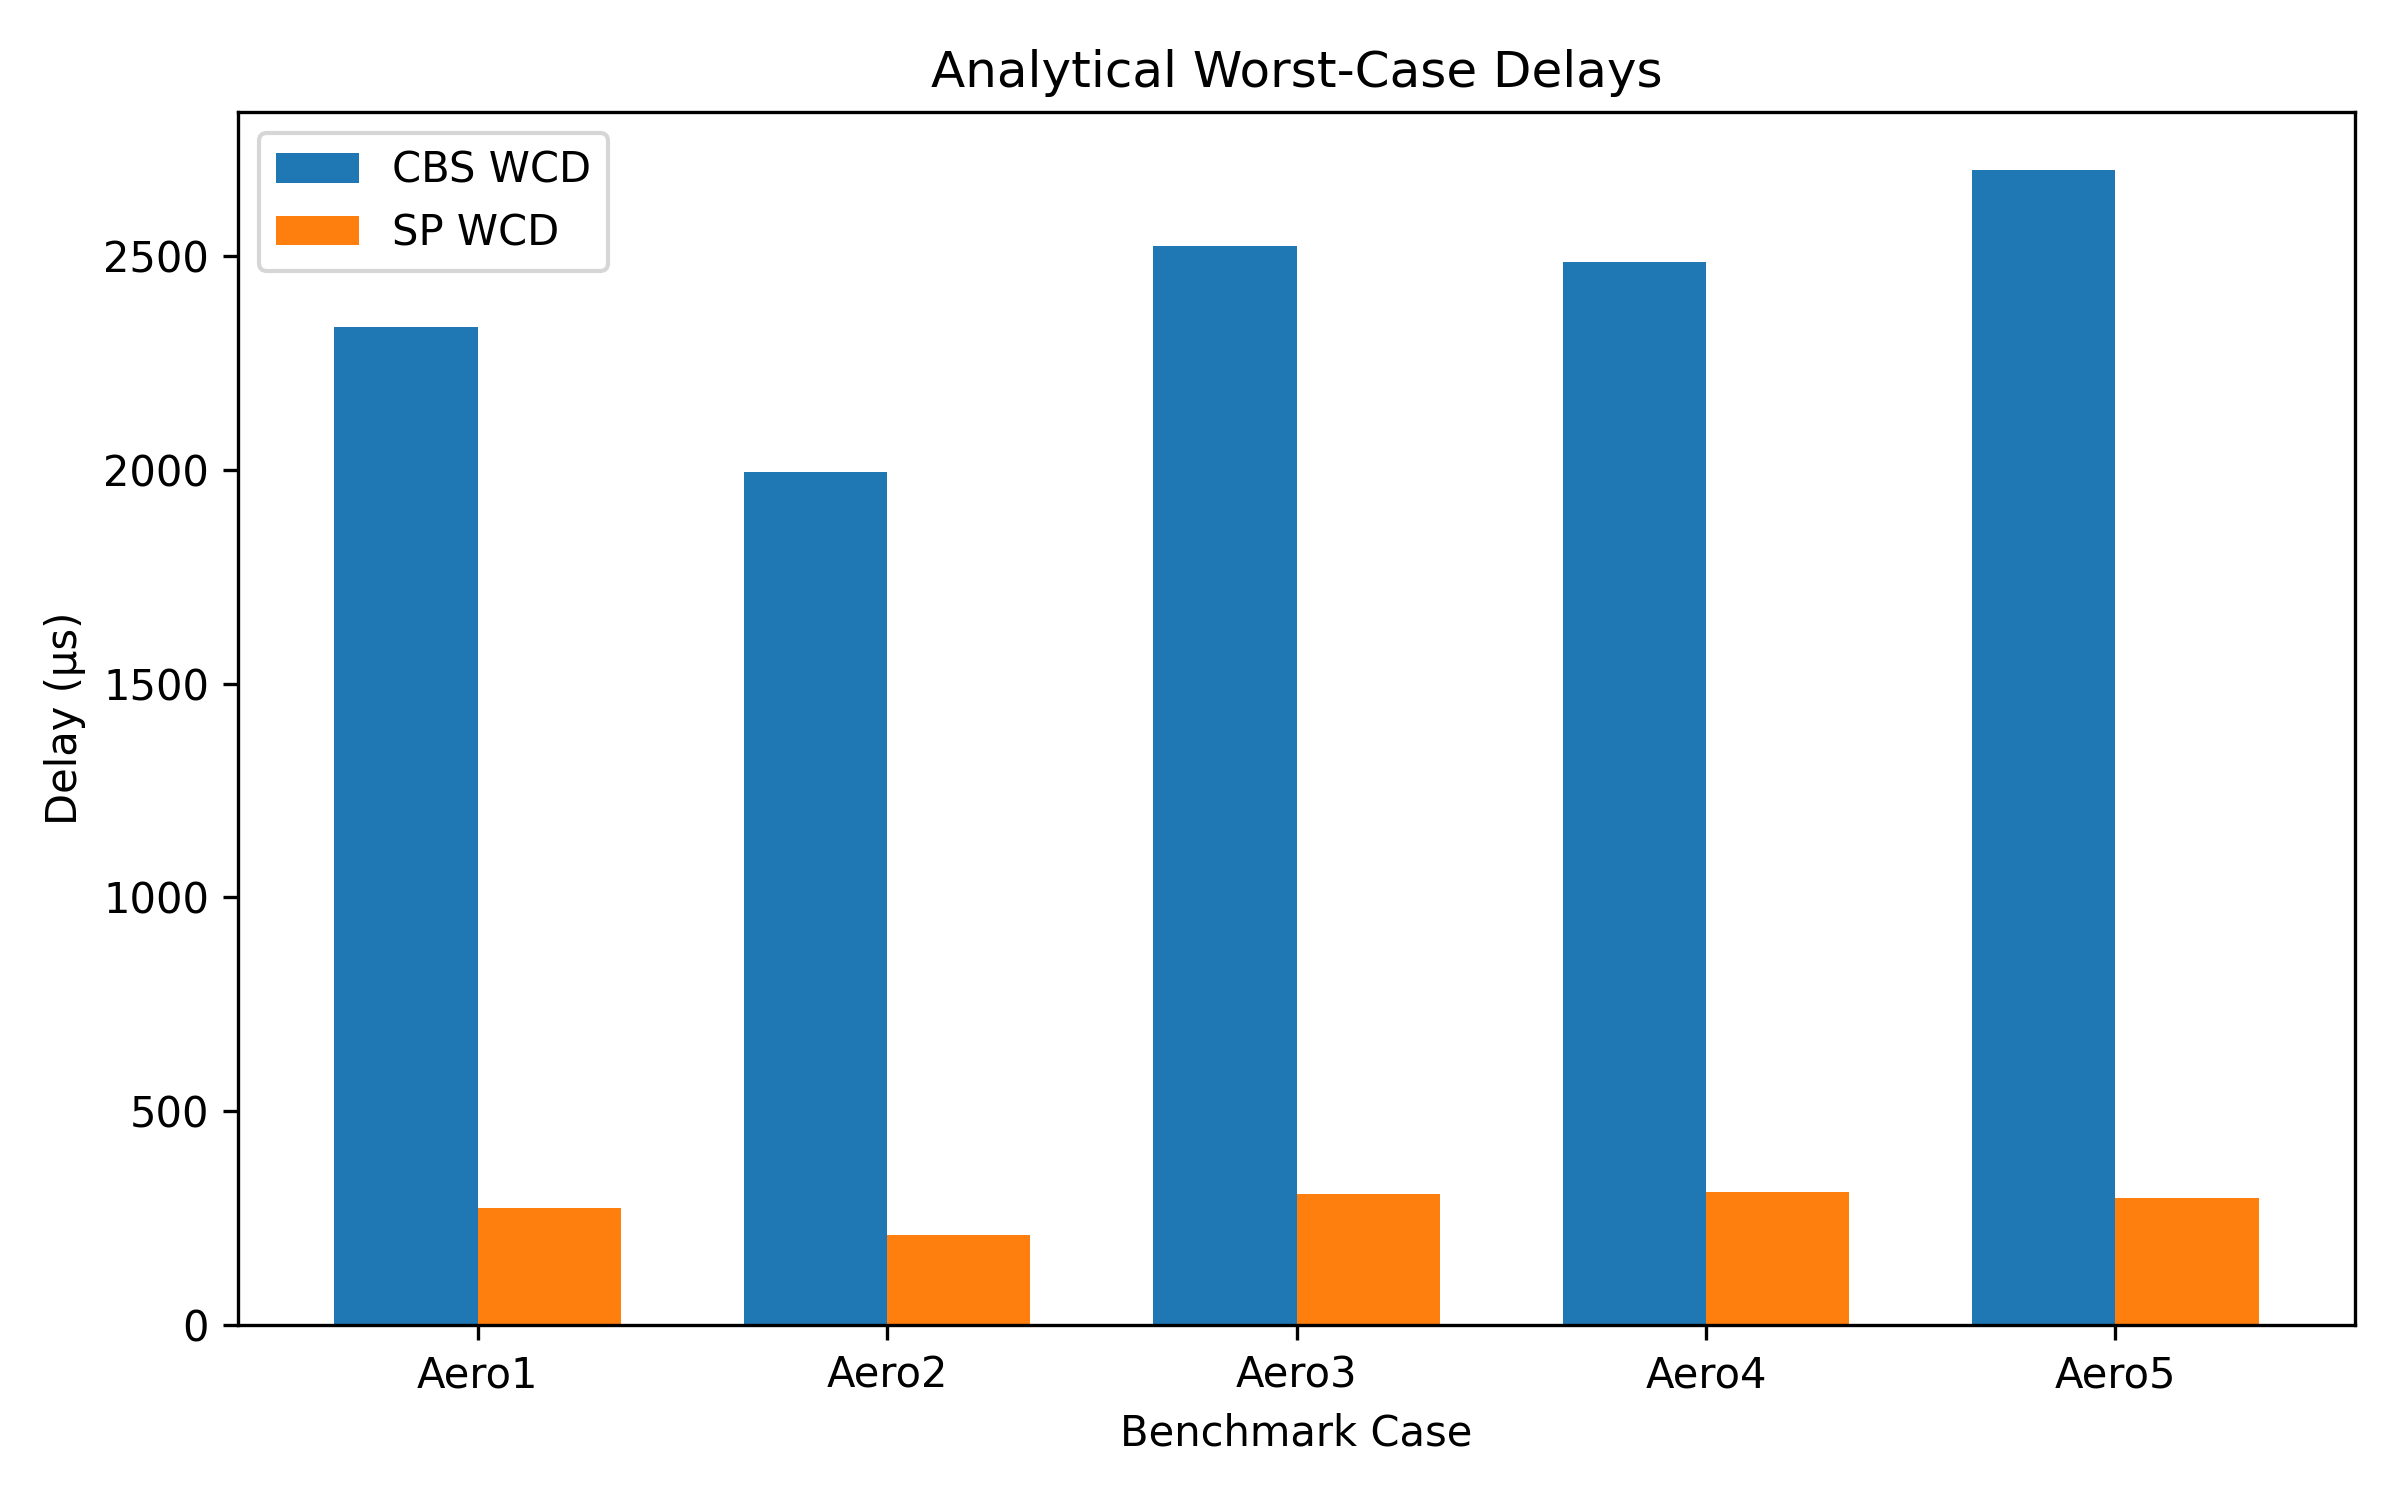
\includegraphics[width=0.8\textwidth]{figures/analytical_delays.png}
    \caption{Analytical worst-case delays (CBS vs.\ SP) for the five aerospace benchmark cases.}
    \label{fig:analytical_delays}
\end{figure}

\begin{figure}[H]
    \centering
    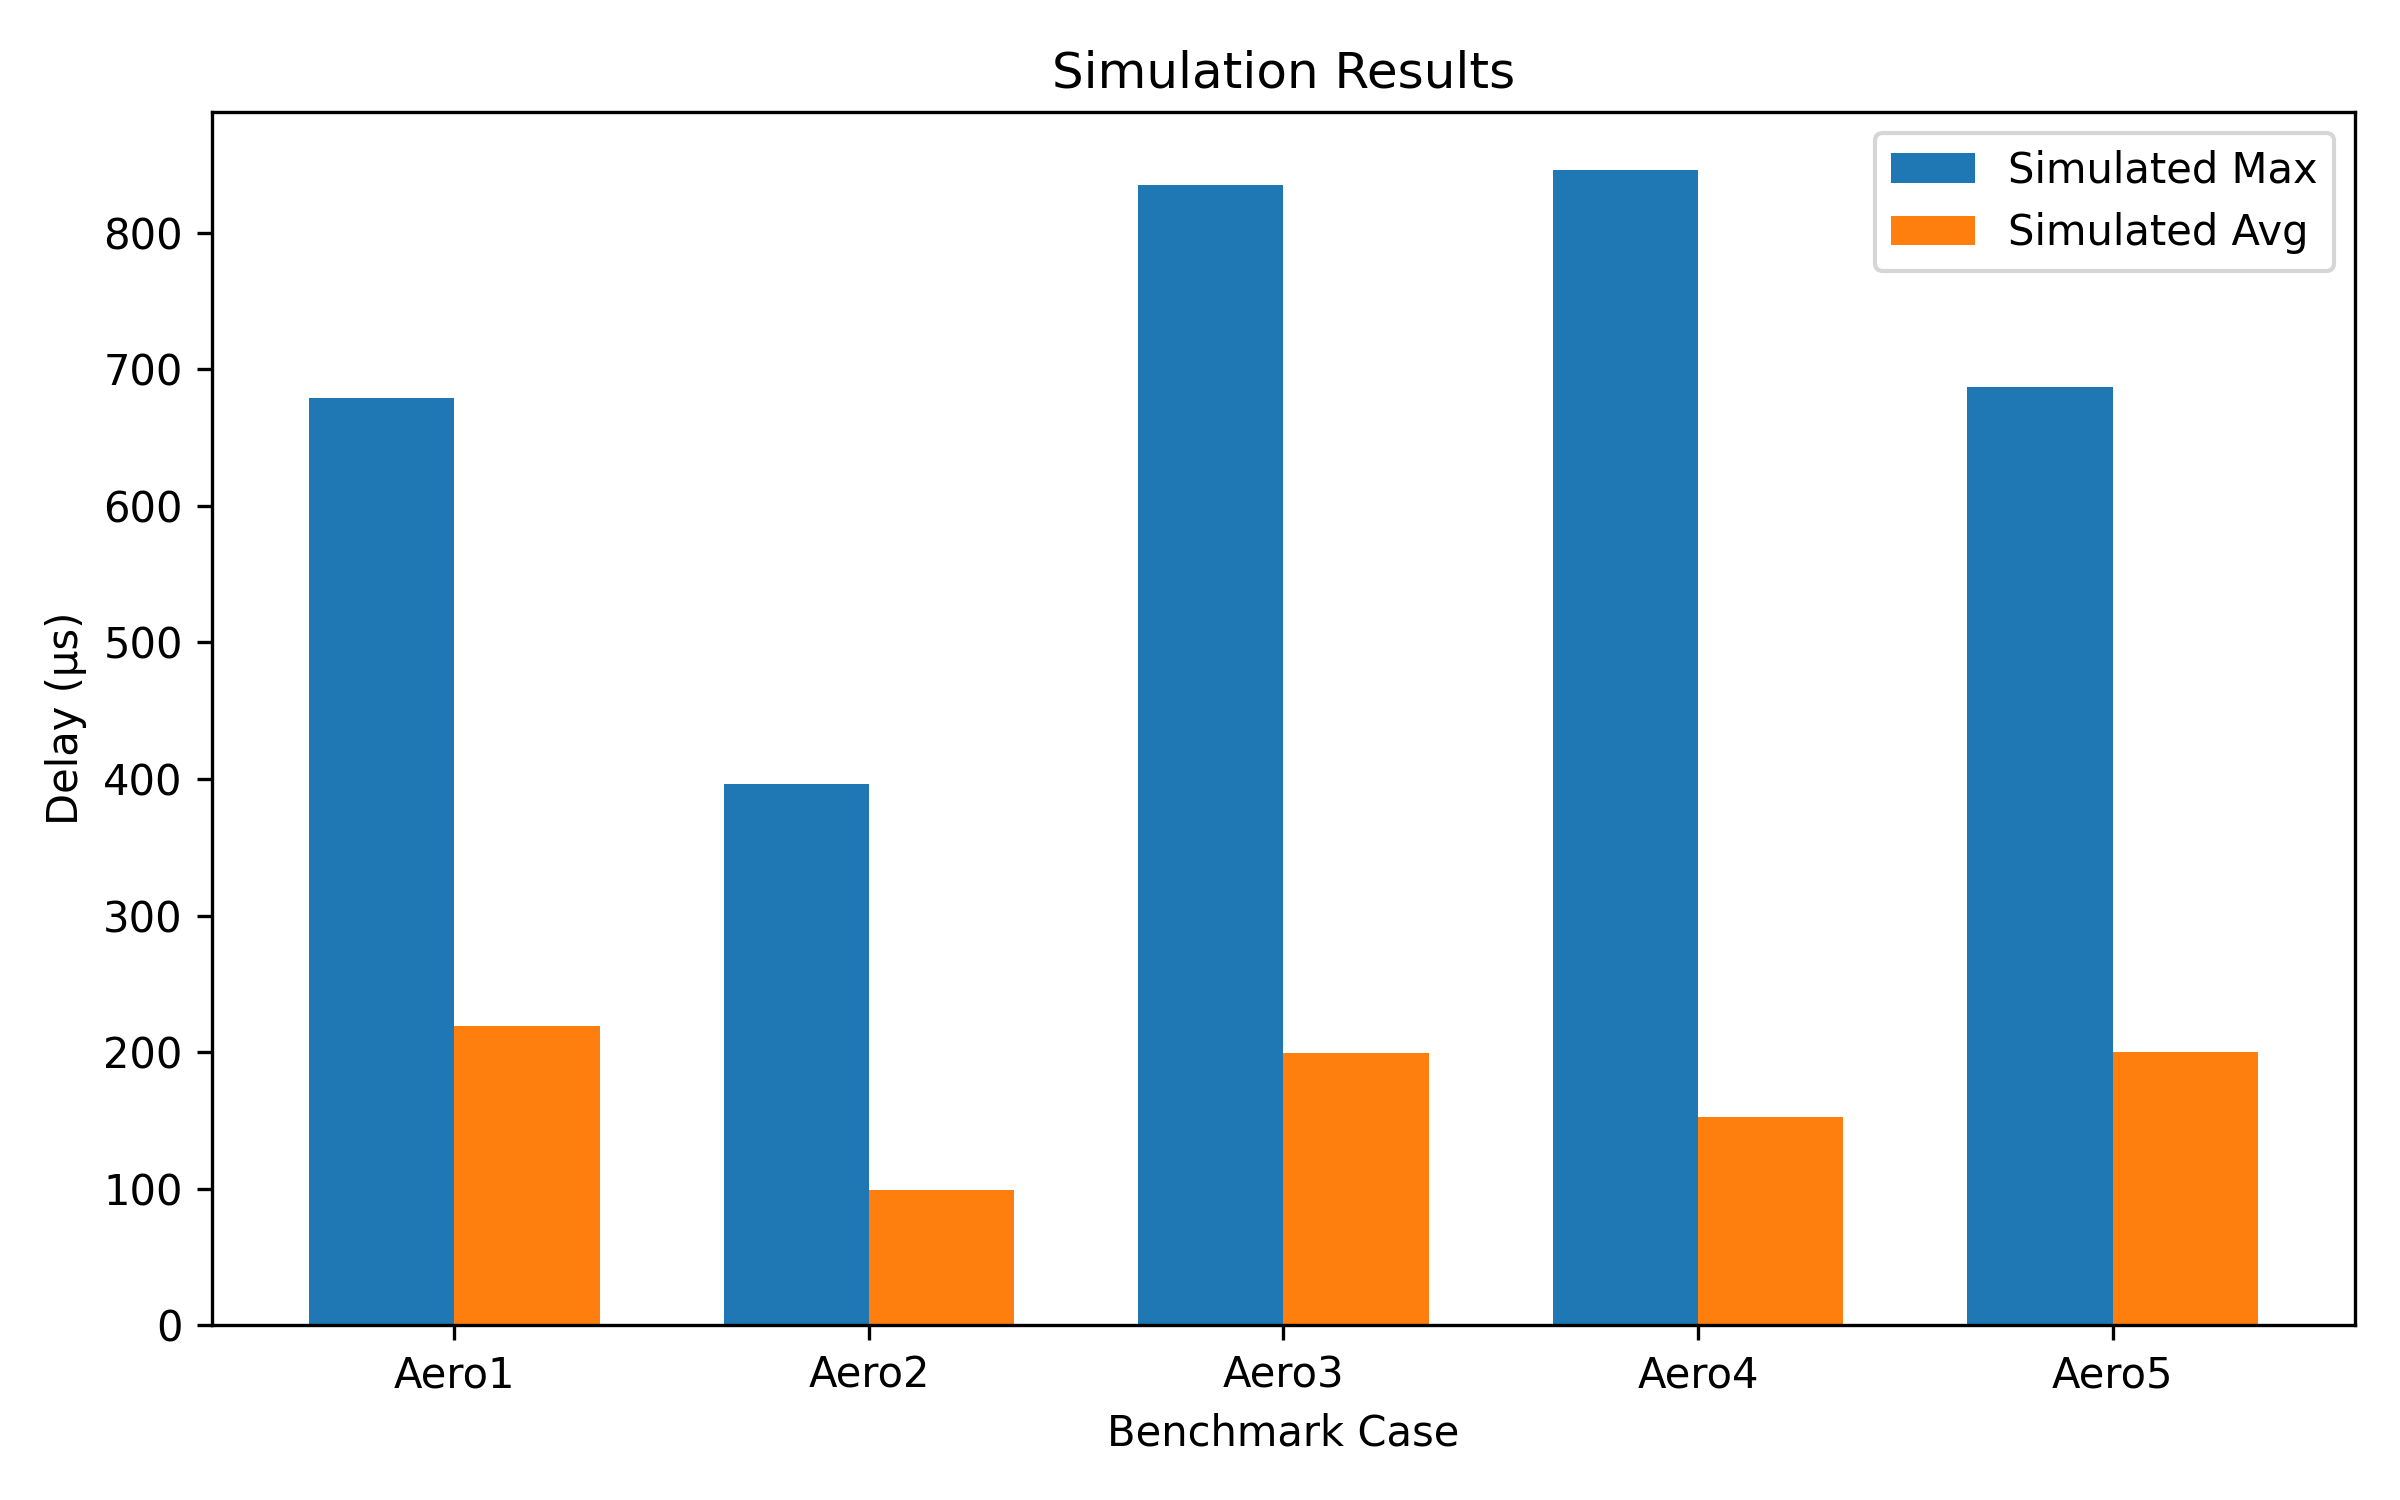
\includegraphics[width=0.8\textwidth]{figures/simulation_results.png}
    \caption{Simulated maximum and average response times for the five aerospace benchmark cases.}
    \label{fig:sim_results}
\end{figure}

\begin{figure}[H]
    \centering
    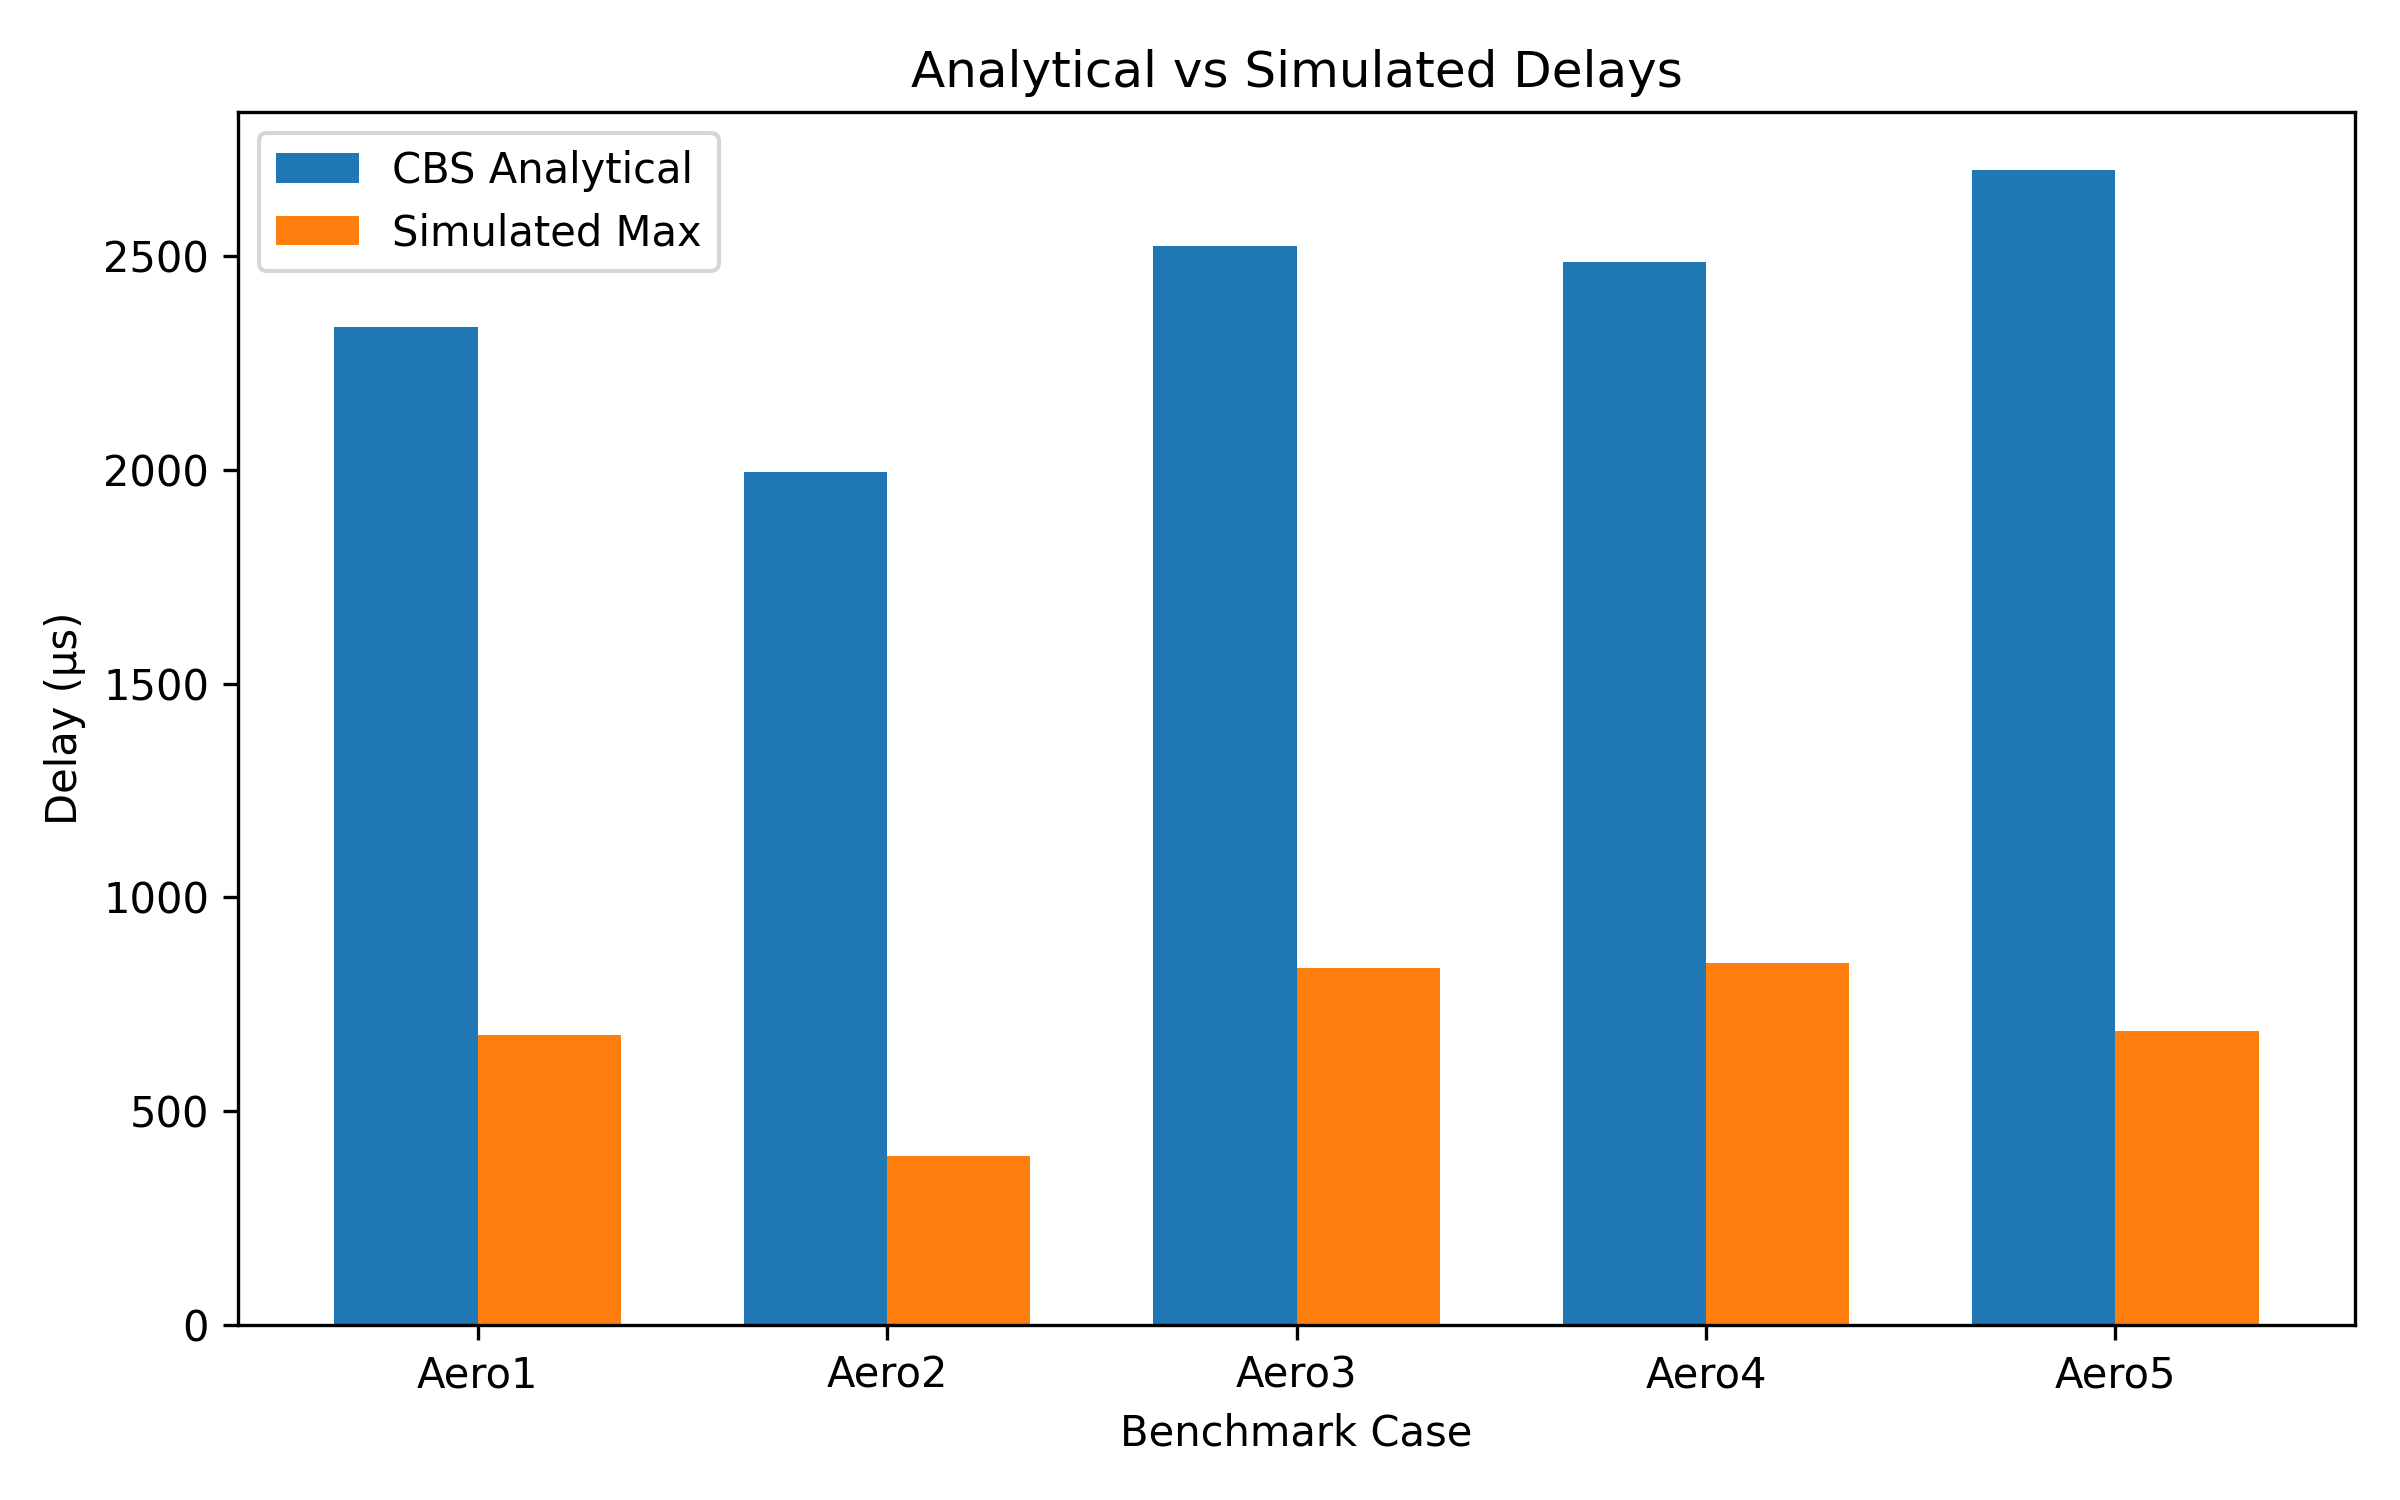
\includegraphics[width=0.8\textwidth]{figures/analytical_vs_simulated.png}
    \caption{Comparison of CBS analytical WCDs and simulated maximum delays for the aerospace benchmarks.}
    \label{fig:ana_vs_sim}
\end{figure}

\begin{figure}[H]
    \centering
    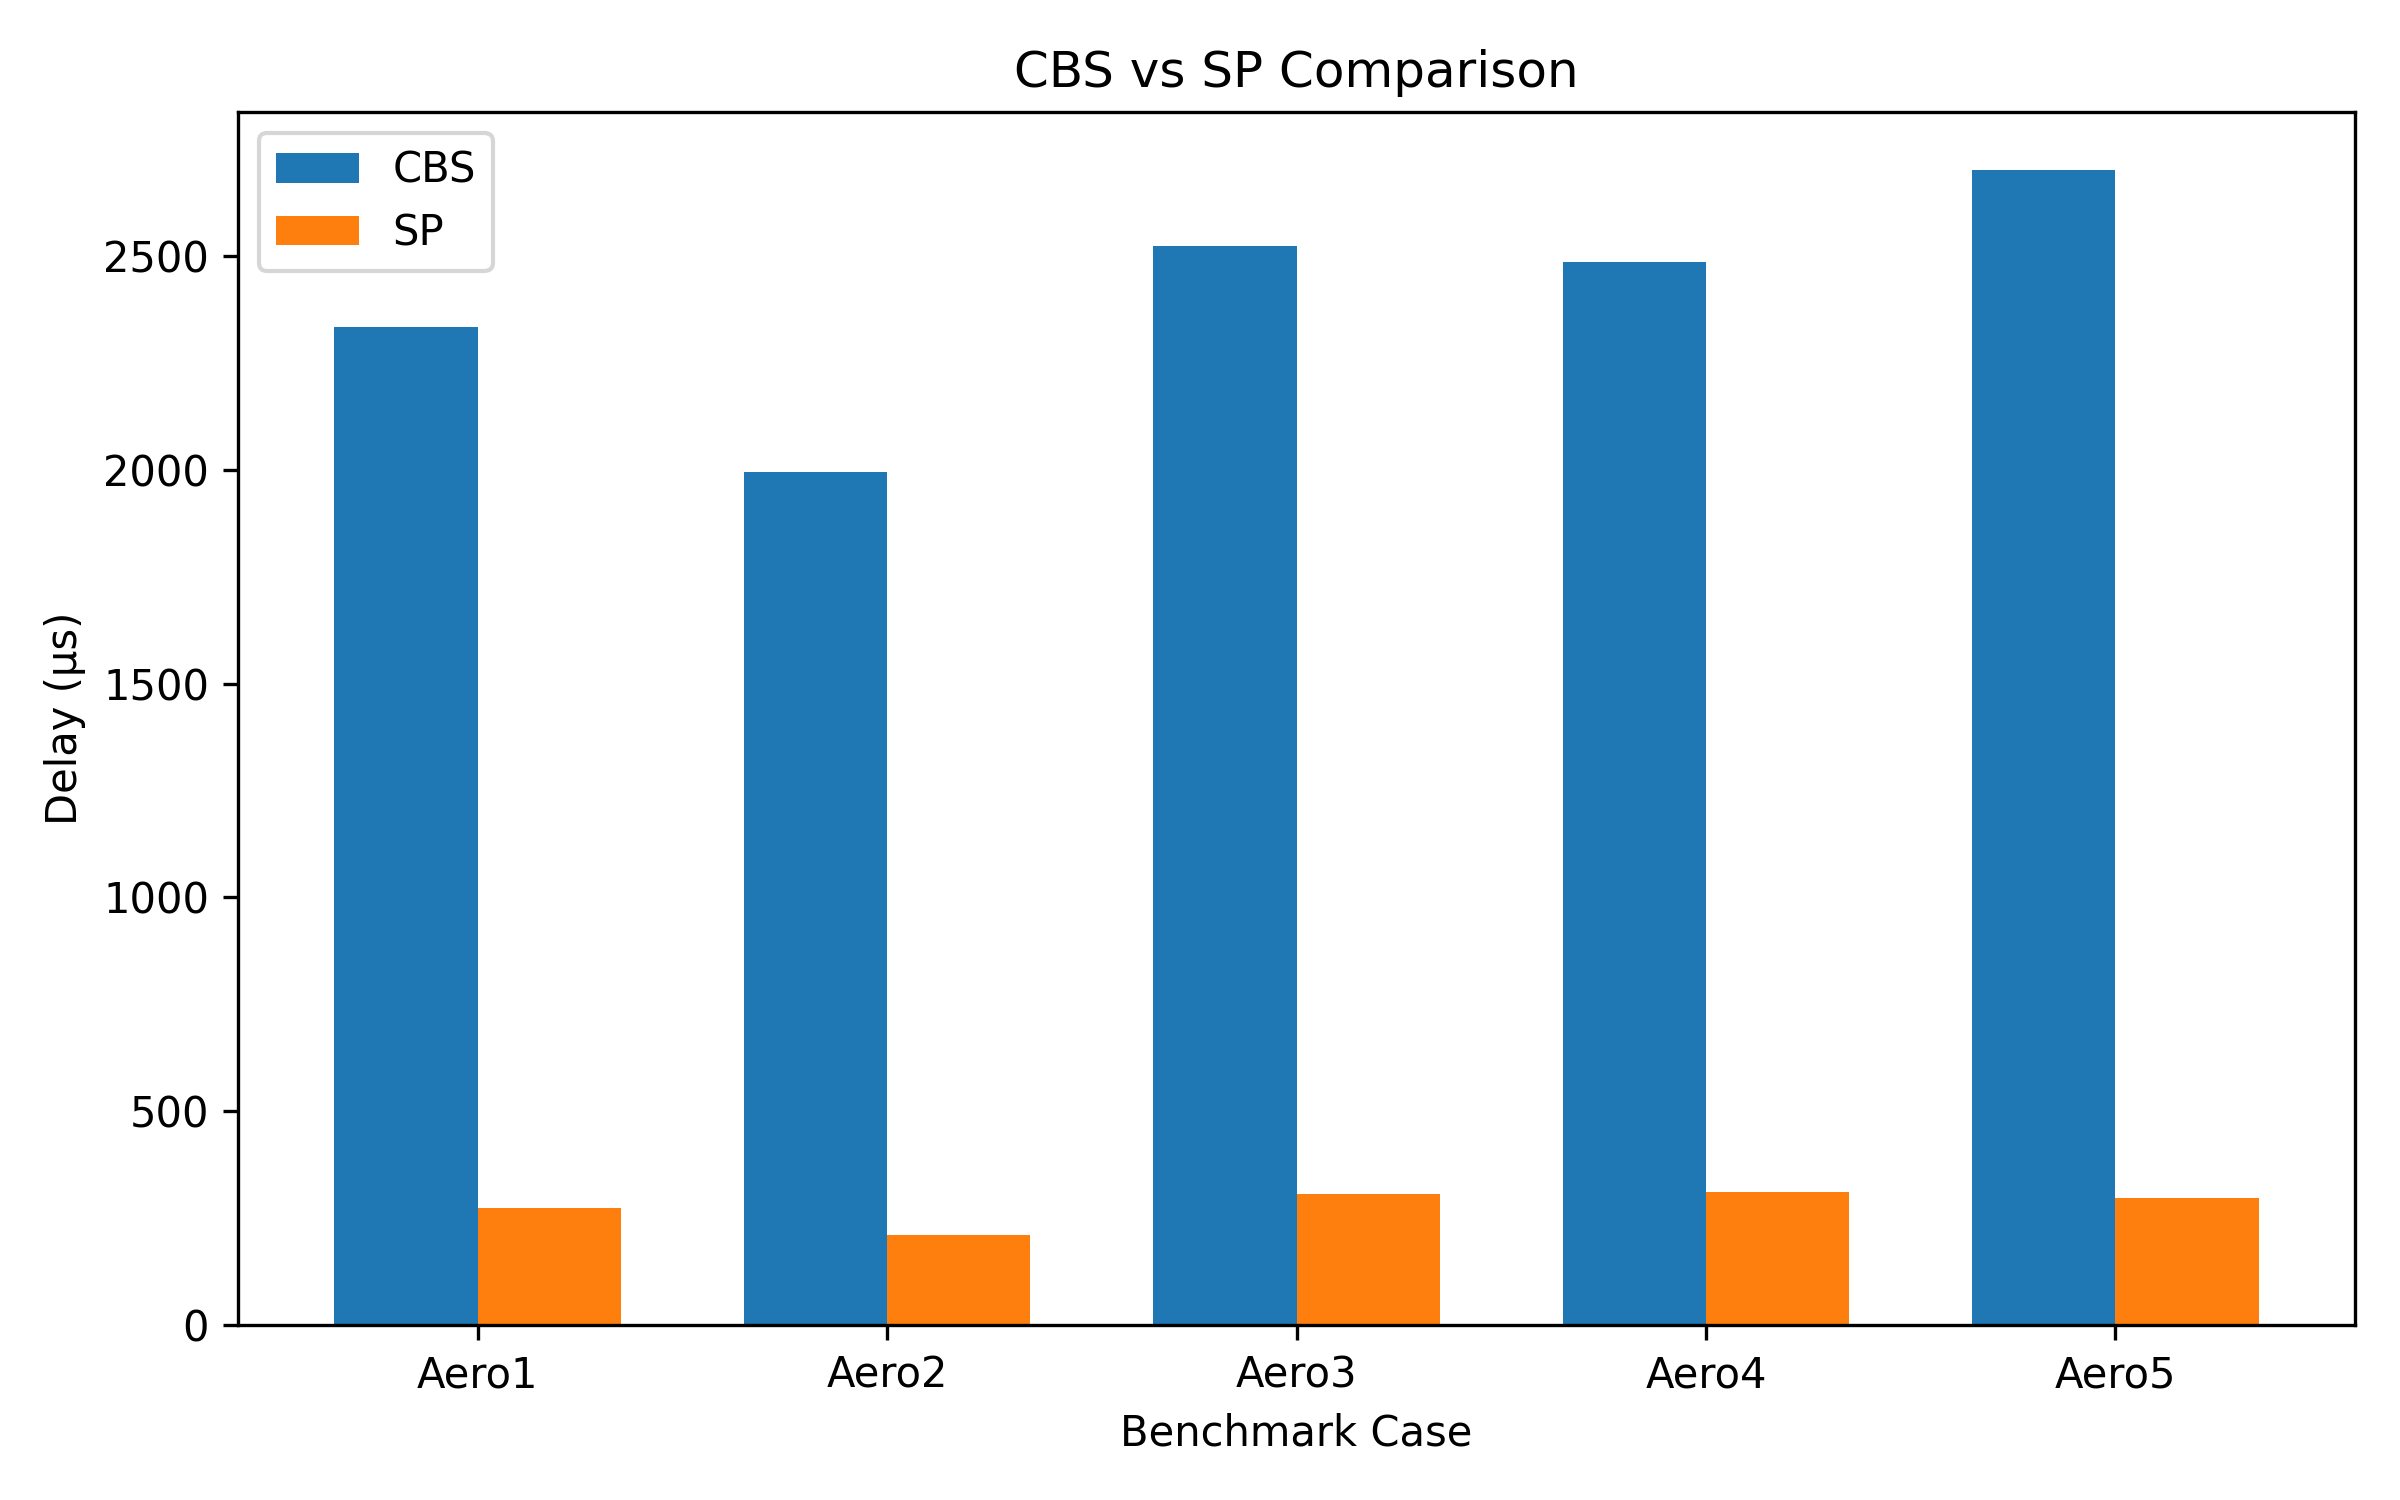
\includegraphics[width=0.8\textwidth]{figures/cbs_vs_sp.png}
    \caption{CBS vs.\ SP analytical worst-case delays for the aerospace benchmarks.}
    \label{fig:cbs_vs_sp}
\end{figure}

Across all five aerospace cases, the CBS analytical WCD is consistently $7$--$9\times$ larger than the SP analytical bound. This gap is expected: CBS introduces credit recovery time (Eq.~\ref{eq:cbs_recovery}) that does not exist under SP. However, the simulated maximum delays lie well below the CBS analytical bound in every case (by a factor of ${\approx}3$--$6\times$), confirming that the analytical model is safe but conservative.

The CBS analytical bound is highest for Aero5 (2701\,\textmu s), which has the largest Class B frames and hence the longest credit recovery delay. Aero2 produces the lowest analytical bound (1996\,\textmu s) and the smallest simulated maximum (397\,\textmu s), suggesting a lighter traffic load relative to the link capacity.

\subsection{Automotive Benchmarks}

Three automotive test cases (Auto1--Auto3) model in-vehicle networks with 1000\,Mbps links and six streams spanning five PCP classes (including BEST-EFFORT streams with no period). The simulation is run only for the periodic streams; BEST-EFFORT streams are excluded because they have no defined period and therefore no periodic arrival pattern. Table~\ref{tab:auto} reports the analytical results only.

\begin{table}[H]
\centering
\caption{Automotive benchmark results — analytical WCDs per stream (\textmu s).}
\label{tab:auto}
\begin{tabular}{llrr}
\toprule
Case & Stream & CBS Analytical & SP Analytical \\
\midrule
\multirow{6}{*}{Auto1}
 & Stream0 & 1617.93 & 4.00   \\
 & Stream1 & 2378.13 & 124.00 \\
 & Stream2 & 2136.33 & 122.80 \\
 & Stream3 & 1967.25 & 245.84 \\
 & Stream4 & 1981.57 & 255.28 \\
 & Stream5 & 1986.45 & 257.68 \\
\midrule
\multirow{6}{*}{Auto2}
 & Stream0 & 1777.25 & 8.64   \\
 & Stream1 & 2408.97 & 127.36 \\
 & Stream2 & 2647.49 & 127.60 \\
 & Stream3 & 2137.13 & 249.44 \\
 & Stream4 & 2133.17 & 257.60 \\
 & Stream5 & 2136.29 & 260.00 \\
\midrule
\multirow{6}{*}{Auto3}
 & Stream0 & 1721.02 & 8.40   \\
 & Stream1 & 2463.62 & 126.80 \\
 & Stream2 & 2349.22 & 128.40 \\
 & Stream3 & 2065.54 & 249.52 \\
 & Stream4 & 2097.14 & 260.48 \\
 & Stream5 & 2669.74 & 380.48 \\
\bottomrule
\end{tabular}
\end{table}

Although the automotive topology uses a 1000\,Mbps link (10$\times$ the aerospace bandwidth), the CBS analytical WCDs remain in the range of 1600--2700\,\textmu s — comparable to the aerospace results. This is because the streams in the automotive cases carry significantly larger frames and the higher-priority interference term $I_i$ (Eq.~\ref{eq:wcd_cbs}) dominates. The SP bounds are very small ($<400$\,\textmu s) because most streams carry only a few bytes and higher-priority classes are sparse.

\subsection{Industrial Benchmarks}

Three industrial test cases (Ind1--Ind3) use 100\,Mbps links with five streams per case, mixing ISOCHRONOUS and BEST-EFFORT traffic. As with automotive, only the isochronous periodic streams are analysed in the simulator.

\begin{table}[H]
\centering
\caption{Industrial benchmark results — analytical WCDs per stream (\textmu s).}
\label{tab:ind}
\begin{tabular}{llrr}
\toprule
Case & Stream & CBS Analytical & SP Analytical \\
\midrule
\multirow{5}{*}{Ind1}
 & Stream0 & 323.44 & 5.60   \\
 & Stream1 & 328.20 & 5.04   \\
 & Stream2 & 323.52 & 5.76   \\
 & Stream3 & 507.84 & 18.80  \\
 & Stream4 & 684.24 & 136.40 \\
\midrule
\multirow{5}{*}{Ind2}
 & Stream0 & 379.91 & 6.64  \\
 & Stream1 & 366.23 & 5.84  \\
 & Stream2 & 370.39 & 4.72  \\
 & Stream3 & 374.11 & 19.60 \\
 & Stream4 & 371.71 & 19.60 \\
\midrule
\multirow{5}{*}{Ind3}
 & Stream0 & 390.11 & 5.36   \\
 & Stream1 & 392.47 & 3.36   \\
 & Stream2 & 392.71 & 3.52   \\
 & Stream3 & 751.03 & 132.24 \\
 & Stream4 & 574.63 & 14.64  \\
\bottomrule
\end{tabular}
\end{table}

Industrial streams are notably smaller (30--1500\,bytes) and carry tighter deadlines than aerospace or automotive. CBS analytical WCDs range from 323\,\textmu s to 751\,\textmu s, well below the aerospace values, reflecting the lower interference burden. The SP bounds are extremely small ($<140$\,\textmu s), confirming that industrial traffic is sparse and lightly loaded.

% ============================================================
\section{Discussion}
\label{sec:discussion}

\subsection{CBS vs.\ Strict Priority}

Across all three domains, the CBS analytical WCD exceeds the SP bound by a factor of roughly $5$--$10\times$. The surplus arises from the credit recovery term (Eq.~\ref{eq:cbs_recovery}): because CBS throttles the aggregate bandwidth of each AVB class to the idle slope fraction $\alpha$, the credit must accumulate between transmissions, adding a latency penalty that SP does not incur.

Despite producing smaller analytical bounds, SP provides \emph{no bandwidth guarantee}: a high-volume Class A burst can starve Class B indefinitely. CBS trades latency headroom for a bounded bandwidth allocation, which is the correct design choice in mixed-criticality TSN deployments where both timeliness and fairness are required.

\subsection{Analytical vs.\ Simulated Delays}

For the aerospace benchmarks, the simulated maximum delay is consistently $3$--$6\times$ below the analytical CBS WCD. Two sources of conservatism explain this gap.

First, our interference model (Eq.~\ref{eq:wcd_cbs}) assumes that \emph{all} higher-priority streams arrive simultaneously at the same port, which is a worst-case assumption that is unlikely to occur in practice when streams originate from different end-stations with independent phase offsets.

Second, the credit recovery estimate (Eq.~\ref{eq:cbs_recovery}) is a first-order approximation; a tighter bound would account for the exact idleSlope/sendSlope dynamics per hop.

The simulation therefore provides a useful \emph{typical-case} reference, but the analytical bound must be used for certification purposes. The TC3 anomaly (Section~\ref{sec:verification}) illustrates the risk of relying solely on simulation: the simulator reveals instability, but only the analytical model can \emph{certify} a bound or — in this case — correctly flag that no finite bound exists.

\subsection{Limitations}

Several simplifications limit the accuracy of the current model.

\begin{itemize}
    \item \textbf{Single-port model.} The simulator models one output port only. A full multi-hop simulator would accumulate per-hop delays with credit states carried across hops.
    \item \textbf{Simplified CBS credit model.} Equation~\ref{eq:cbs_recovery} is a conservative upper bound on the credit recovery time; the standard IEEE 802.1Qav analysis \cite{ieee8021qav} provides tighter formulae that account for the exact slope parameters and frame sizes.
    \item \textbf{BEST-EFFORT streams excluded.} Streams with \texttt{null} period (automotive and industrial) are not included in the simulation. In practice, best-effort traffic contributes non-zero queuing delay and its stochastic behaviour should be modelled (e.g.\ via token-bucket characterisation).
    \item \textbf{Fixed phase offset.} The simulator releases all streams at $t=0$. Staggered offsets, as used in real deployments (e.g.\ via gPTP offset assignment), would reduce worst-case contention.
\end{itemize}

% ============================================================
\section{Conclusion}
\label{sec:conclusion}

We have implemented and evaluated a worst-case delay analysis framework for CBS-scheduled TSN networks. The analytical model provides safe upper bounds on end-to-end delays and correctly predicts overload conditions (as demonstrated in TC3). Comparison against an event-driven CBS simulator confirms that the bounds are conservative by a factor of 3--6$\times$ under typical aerospace traffic patterns, which is acceptable for a first-order design-space exploration tool.

Across the three benchmark domains, the CBS WCDs are significantly higher than SP bounds, but SP cannot guarantee bandwidth isolation. CBS is therefore the preferred shaping discipline for mixed-criticality TSN networks. Future work should extend the analytical model to a proper multi-hop network calculus formulation and incorporate stochastic characterisation of best-effort traffic.
